
% this file is called up by thesis.tex
% content in this file will be fed into the main document

%: ----------------------- introduction file header -----------------------
% the code below specifies where the figures are stored
\graphicspath{{5/figures/}}

\chapter{Automatic Chord Estimation}
\label{chp:chord_estimation}

\section{Context}
\label{sec:context}

% Timbre, though hard to define, is relatively constrained
Even though a satisfactory definition remains elusive, it is important to recognize that the perception of timbre is tightly coupled with its physical acoustic stimulus.
Therefore, it shares the trait with other sensory phenomena, like pitch or loudness, that all information necessary to model human experience is contained within a signal representation.
These kinds of low-level percepts are literal in nature, especially when compared to more abstract concepts like artist recognition or estimating tension.
As it is a particular goal of this work to explore how deep learning methods can be applied to the murky waters of music analysis, we now turn our attention to the problem of automatically transcribing chords from polyphonic music recordings.

\subsection{Musical Foundations}
\label{subsec:musical_foundations}

In lieu of a general, perhaps impossible, definition of ``music'', we instead arrive at a confined concept through a set of constraints.
Here, we are primarily interested in the tradition of tonal Western music, with a particular focus on popular contemporary music from the last century, built upon a 12-Tone Equal Temperament (12-TET) tuning system.
Furthermore, music typically lives in two domains: one, \emph{symbolic}, in the form of scores, MIDI, or countless other forms of abstract musical representations; and two, rendered via synthesis as \emph{sound signals}, which may be transmitted through physical space as acoustic waves or stored in a persistent state as static information, e.g. a sound recording.
% Framed in this way, this work is concerned with the machine audition of music, whereby sound signals are transformed into some form of symbolic notation.

% Dimensions of music
Continuing, it can be said that there are three fundamental dimensions to this kind of music:

\begin{itemize}
\item Rhythm: the understanding of loudness as a function of time.
\item Harmony: the understanding of pitch as a function of time.
\item Timbre: the understanding of sources as a function of time.
\end{itemize}

In all three dimensions, observable signal qualities give rise to sensory percepts.
``Loudness'' is defined as the phenomena whereby sound stimuli can be compared with respect to intensity, and is closely related to signal power.
Orthogonally, ``pitch'' is defined as the phenomena whereby a sound stimulus can be matched to the frequency of a pure sinusoid, and is a result of the harmonic components, or partials, found in complex sounds.
Lastly, and in spite of timbre's ambiguous nature, we constrain it here to mean the phenomena by which concurrent voices may be identified and differentiated in a single sound stimulus.

% Historical context -> Harmonic analysis
Contextualizing briefly, theorists have long sought to characterize musical works via analysis and reduction as a means to understanding.
With sound recording being a relatively modern invention on the timescale of music history, much effort to this end has been invested in the analysis of symbolic notation, or scores.
%, which cleanly delineate the three dimensions described previously; an example of this is given in Figure \ref{fig:notated_music}.
Evolving over time from the counterpoint of J. S. Bach to the functional analysis of Heinrich Schenker or more recently Fred Lehrdal, traditional musical analysis revolves heavily around the harmonic facets of a musical piece by marginalizing the dimensions of rhythm and timbre.
As a result, the harmonic language of ``chords'' developed as a rich yet compact vocabulary to describe a piece of music; an instance of such a harmonic analysis is given in Figure \ref{fig:notated_music}.

% Attempts to define a chord
Unfortunately, what comprises a chord is open to some interpretation, and no singular definition exists.
For example, \cite{McVicar2013} collects three possible definitions of a chord, restated here:

\begin{enumerate}
\item \emph{Everyone agrees that \emph{chord} is used for a group of musical tones.}
\item \emph{Two or more notes sounding simultaneously are known as a chord.}
\item \emph{Three or more pitches sounded simultaneously or functioning as if sounded simultaneously.}
\end{enumerate}

% Pitch and notes
Alternatively, \cite{Harte2010} expands the scope of (2) in order to describe a wider space of music, ``allow[ing] a chord to comprise zero or more notes.''
It is both important and interesting to observe the concepts of \emph{pitch}, \emph{tone}, and \emph{note} are used interchangeably.
For clarity, a tone is a perceptual object with a pitch, whereas a note is a musical object that may be realized as sound subject to a given tuning system.
The relationship between the two in equal temperament is defined as the following:

\begin{equation}
\label{eq:tuning}
f_{pitch} = f_{tuning} * 2 \exp((n_{index} - 48) / N)
\end{equation}

\noindent~where $N$ is the number of notes per octave, $n_{index}$ is an integer note index, $f_{tuning}$ is the frequency, in Hertz, of a reference tone, and $f_{pitch}$ is the resulting frequency, in Hertz, of the corresponding note.
An \emph{octave} is defined as the doubling of a quantity, and exhibits a special relationship in human perception by which two tones, differeing by an integer power of 2, are perceived as similar; this phenomena is referred to as octave equivalence \cite{?}.

Therefore, in 12-TET, it is useful to name the unique pitch classes per octave, given in the following ordered set, $\mathcal{P}$:

\begin{equation}
\label{eq:pitch_classes}
\mathcal{P} = \{C, C\sharp / D\flat, D, D\sharp / E\flat, E, F, F\sharp / G\flat, G, G\sharp / A\flat, A, A\sharp / B\flat, B\}
\end{equation}

An absolute note name, consisting of a pitch class and an octave index, is given by the following as a function of absolute note index, such that $n_{index}=0~\to~C0$:

\begin{equation}
(\mathcal{P}[mod(n_{index}, 12)], \lfloor~n_{index} / 12~\rfloor)
\end{equation}

In contemporary music, standard concert tuning equates $A4=440Hz$; classically, the tuning frequency is defined such that it falls in the performance range of a majority of instruments to be matched exactly, and hence the offset in Eq. \ref{eq:tuning}.
Were this tuning frequency constant, the notions of pitch and note would be equivalent; it should be noted, however, this is not always the case.

% Chord composition
It may be difficult or ambiguous to infer the significance of a pitch collection by notes alone, and therefore chords are typically named according to three criteria: the relative intervals between the notes it contains, the note corresponding to the \emph{root}, and its overall relationship to the local \emph{key}.
Intervals describe the integer distance between notes: adjacent notes or pitch classes is referred to as a \emph{semitone}, with a step size of 1, whereas a step size of 2 is known as a \emph{whole tone}.
A ``root'' is the note in a chord that serves as a point of \emph{internal} harmonic stability; conversely, a ``key'' is itself a chord which serves as a point of \emph{external} harmonic stability.
Therefore, as we will shortly see, the name a chord takes can change based solely on contextual information.

% Chord Names
The final piece of information necessary before we can discuss chord spellings is the concept of the diatonic scale, upon which the vast majority of Western harmony is built.
It is expressed here as an ordered set of intervals ($T$ for whole tone, $s$ for semitone) and relative semitone degrees:

\begin{equation}
\mathcal{D}_{intervals} = \{T, T, s, T, T, T, s\} \\
\mathcal{D}_{semitones} = \{0, 2, 4, 5, 7, 9, 11\}
\end{equation}

\noindent Using the diatonic scale to index a set of pitch classes in \ref{eq:pitch_classes}, one arrives at a \emph{major} scale, where the starting note is referred to as the \emph{tonic}.
In the key of $C$, this takes the following form:

\begin{equation}
\mathcal{C}_{major} = \{C, D, E, F, G, A, B\}
\end{equation}

We can now build our first chord \emph{quality}, the major triad, comprised of the first, third, and fifth major scale degrees:

\begin{equation}
\mathcal{M}_{semitones} = \{0, 4, 7\} \\
\text{e.g. in the key of} C, C:maj = \{C, E, G\}
\end{equation}

Note that a triad is any chord comprised of three notes; later, we will also consider tetrads, or chords consisting of four notes.
Additionaly, we introduce the concept of a quality here to describe the root-invariant components of a chord, i.e. the intervals.

Rotating the diatonic scale produces other \emph{modes}, of which the most common is minor, resulting from a circular shift of 3:

\begin{equation}
\mathcal{m}_{intervals} = \{T, s, T, T, s, T, T\} \\
\mathcal{m}_{semitones} = \{0, 2, 3, 5, 7, 8, 10\}
\end{equation}

\noindent Starting this time from $A$, we arrive at the resulting minor scale:

\begin{equation}
\mathcal{A}_{minor} = \{A, B, C, D, E, F, G\}
\end{equation}

We can now build our second chord \emph{quality}, the minor triad, comprised of the first, third, and fifth \emph{minor} scale degrees:

\begin{equation}
\mathcal{m}_{semitones} = \{0, 3, 7\} \\
\text{e.g. in the key of} A,~A:min = \{A, C, E\}
\end{equation}

% Chord Observations
Here, a few important observations should be made.
First, the scales of $\mathcal{C}_{major}$ and $\mathcal{A}_{minor}$ are comprised of the exact same pitch classes, differing only as a function of where the scale begins; these are known as relative major and minor scales, respectively.
Additionally, a triad can be formed taking any scale degree as its root, and as a result different keys will share chords.

% Why is it so hard to define a chord? Let's look at some examples
Having covered the basic elements of Western tonal theory, it is now possible to develop a better understanding of the variation and difficulty in defining a chord by exploring a few specific, if simple, examples.
The one invariant property shared by all defintions named previously is the idea that a pitch collection may be understood as a single entity.
The time span over which this phenomena may unfold, however, is flexible.
To illustrate the point, consider the three bars notated in Figure \ref{fig:expanded_major}, where a major chord is written as a true simultaneity, an arpeggiation, and as an series of non-overlapping quarter notes, respectively.
In this instance, the degree of overlap in time is expanded until it no longer exists, and yet the collection of notes continues to function as a coherent harmonic object.

\begin{figure}[t]
\centering
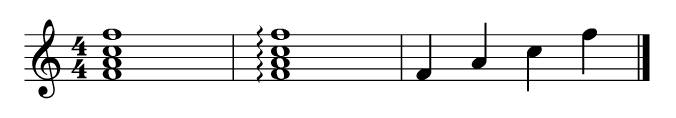
\includegraphics[width=5in]{expanded_major}
\caption{writeme}
\label{fig:expanded_major}
\end{figure}

On the other hand, as shown in Figure \ref{fig:nonchord_tones}, the simultaneous sounding of different notes does not necessarily give rise to the perception of different chords.
Here, a major triad is sustained under the first several degrees of its scale.
While three notes in the upper voice are contained in the C:maj triad, the other three --the D, F, and A-- are known as ``nonchord'' tones.
These ``extra'' tones, however, can be explained away in the overall harmonic scene, as they fall on metrically weak beats, are comparatively short in duration, and are quickly resolved to chord tones.
As a result, they do not contribute significantly to the harmonic center of the phrase, and the bar is still understood as a stable C:maj.


\begin{figure}[t]
\centering
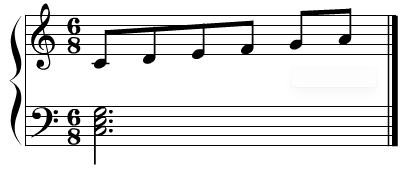
\includegraphics[width=3in]{nonchord_tones}
\caption{writeme}
\label{fig:nonchord_tones}
\end{figure}

A final example, shown in Figure \ref{fig:fifths_context}, demonstrates the role that context and the perception of key can play on the understanding of a chord.
Here, two diatonic scales --one major and the other minor-- descend to identical pitch combinations, consisting of the tonic, fifth, and octave degrees.
Therefore, even though the chords are absent a third scale degree, they are perceived as having the quality of the leading context, being major and minor respectively.
Though similar in principle to that of Figure \ref{fig:expanded_major}, this example serves to demonstrate that ambiguous simultaneities can be resolved by incorporating contextual information.

% Real music on the other hand, like the first system of a Beethoven string quartet given in Figure \ref{fig:beethoven}, can be remarkably complex and require a good deal of expertise to complete a formal analysis of the score.
% Skilled musicans are quite robust in the ability to assign chord labels to musical scenes despite an occasionally opaque decision making process, and it is an exciting challenge to produce a computational system with a similar capacity.
% However, as discussed in the following section, the topic is also motivated by a long research tradition in MIR.

% \begin{figure}[!t]
% \centering
% 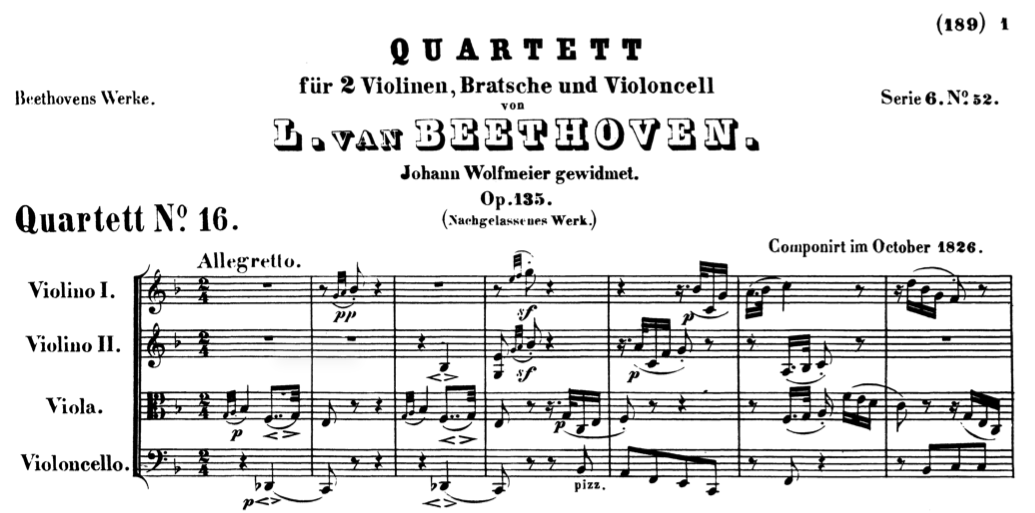
\includegraphics[width=5in]{beethoven}
% \caption{writeme}
% \label{fig:beethoven}
% \end{figure}

\subsection{Chord Syntax}
\label{sec:chord_syntax}

It is a pragmatic but ultimately necessary prerquisite step to define a standard syntax for consistently referencing and describing chords.
Much of the pioneering work in this space was performed by Harte \cite{Harte2010}, and many of these conventions are utilized here.
For clarity, we stylize chords in this syntax with a fixed-width font, e.g. \texttt{A:min}.

Firstly, Harte's general chord notation is described by the following four-part symbolic description:

\begin{equation}
\{r\}:\{q\}(i)/\{b\}
\end{equation}

\noindent Every chord name begins with a root $r$ in the form of a valid pitch class, optionally modified by zero or more sharps or flats, or one of two reserved characters: \texttt{N} for the ``null'' no-chord condition, or \texttt{X} for the special case in which the musical content cannot be described harmonically.

The root name is potentially followed by a quality shorthand, $q$, separated by a colon and implying a particular set of note intervals.
Though there are a large number of possible chord qualities, this is often limited to a particular subset in practice.
Those considered in this work are indicated in the following table:

\begin{table}[h]
\begin{center}
\caption{Chord quality names and corresponding relative semitones.}
\begin{tabular}{l | c | c}
Name & Shorthand & Semitones \\
\hline
Major & \texttt{maj} & $\{0, 4, 7\}$ \\
Minor & \texttt{min} & $\{0, 3, 7\}$ \\
Major 7 & \texttt{maj7} & $\{0, 4, 7, 11\}$ \\
Minor 7 & \texttt{min7} & $\{0, 3, 7, 10\}$ \\
Dominant 7 & \texttt{7} & $\{0, 4, 7, 10\}$ \\
Major 6 & \texttt{maj6} & $\{0, 4, 7, 9\}$ \\
Minor 6 & \texttt{min6} & $\{0, 3, 7, 9\}$ \\
Diminished & \texttt{dim} & $\{0, 3, 6\}$ \\
Augmented & \texttt{aug} & $\{0, 4, 8\}$ \\
Suspended 2$^{nd}$ & \texttt{sus2} & $\{0, 2, 7\}$ \\
Suspended 4$^{th}$ & \texttt{sus4} & $\{0, 5, 7\}$ \\
Fully-diminished 7 & \texttt{dim7} & $\{0, 3, 6, 9\}$ \\
Half-diminished 7 & \texttt{hdim7} & $\{0, 3, 6, 10\}$ \\
\hline
\end{tabular}
\label{tab:qualities}
\end{center}
\end{table}


The third field provides an interval set, $i$, wrapped by parentheses.
In practice, there are two reasons for representing information intervallically.
One such instance is, through a combination of additional degrees and asterisks, the modification of a quality shorthand in order to represent a non-standard, but related, chord.
An example of this might be the chord name \texttt{A:min(*b3, 7)}, which means that the minor third ($C$) is absent, but a major 7 ($A\flat$) has been added.
The other instance occurs when the intervals are certain but the quality is ambiguous, such as \texttt{C:(1, 5)}; note that this is a valid spelling of the chord shown in Figure \ref{fig:powerchord_context}.

The final field of this chord syntax is the bass interval, $b$, which indicates the scale degree at the bottom of the chord.
Typically this is also the root of the chord, and is implied in the absence of an explicit bass interval.
However, it is necessary to state that the scale degrees of the chord --given by the quality shorthand and the interval set-- can be further augmented by the inclusion of a bass interval.
For example, the chords \texttt{C:maj/b7} and \texttt{C:7} would be understood as containing the same pitch classes, but are spelled quite differently.


\subsection{Motivation}
\label{sec:motivation}

% Historical Context
Even from the earliest efforts in content-based music informatics research, automatic music transcription has stood as one of the Holy Grails of the field.
Over time, however, it would prove exceptionally difficult, and fracture into a variety of smaller, and hopefully more manageable, subtopics.
As a result, automatic chord estimation materialized as one such task, now receiving healthy attention for more than a decade, and established as a benchmark challenge at the annual MIReX event \footnote{{http://www.music-ir.org/mirex/wiki/MIREX\_HOME}}.

% Applications
% - People
Given the prerequisite skill necessary to produce these transcriptions manually, there is considerable motivation to develop automated systems capable of reliably performing this task.
As evidenced by large online communities surrounding websites like e-chords\footnote{http://www.e-chords.com} or Ultimate Guitar\footnote{http://www.ultimate-guitar.com}, countless individuals invest considerable time and effort in the curation and consumption of popular music transcriptions.
Often this is driven by desire to learn and perform music for which symbolic notation does not exist.
Conversely, automatic chord transcription systems would be particularly useful in the areas of composition, recording, and production.
Furthermore, the curation of this content would enable large-scale musicological analysis of contemporary music.

% MIR Systems
In addition to the concerns of individual users, computational systems capable of reliable chord transcription are directly useful inside the domain of content-based MIR.
Chords can serve as a robust mid-level representation with which to build systems and extract higher level musical knowledge.
This has been used in the space of cover song retrieval \cite{Juan?}, navigating large collections \cite{alan?}, and genre recognition \cite{anglade}.
Such systems would also facilitate data collection for other tasks, aiding in visualization and other facets of music transcription.

% Theoretical merit
From a more philosophical perspective, the identification of chords is also intriguing as an intelligent musical behavior, being a high level cognitive process that is often open to multiple interpretations between knowledgable experts.
Experiential bias of the annotator may manifest in the subjective decisions made by an observer, where a pianist may arrive at a different harmonic analysis than that of a guitarist due to how a collection of notes might be produced.
Lastly, the knowledge and skill of the one recognizing chords in music will affect the resulting interpretations.
Beginners will likely prefer simple or more common descriptions, whereas experts will be more aware of complex nuances and have better command over a larger harmonic vocabulary.


\subsection{Limitations}
\label{sec:limitations}
% Limitations
It should be acknowledged that such an inquiry is subject to certain limitations, and there are two worth mentioning here.
The first derives from the philosophical limits of objective truth in an inherently subjective task.
As outlined previously, the definition of a chord is open to interpretation, and may be influenced by individual experience, degree of skill, and intended purpose.
This begs a potentially damning question: What hope is there for an automatic algorithm if you can't define your concepts?
Furthermore, ``expert'' annotations used in the development and evaluation of computational systems is based on the assumption that all subjects apply the same rules to some unknown degree of consistency.

The second notable limitation is related to the validity and relevance of chords as a means to describe musical content.
Even in the constrained space of Western tonal music set forth here, not all musical works will be well-described by the language of harmonic analysis.
Therefore a chord transcription may be a poor approach toward representing such a piece of music.
In some cases an alternative approach to analysis, such as voice leading, might make more sense; in others, such as rap or math rock, a lack of clearly structured harmonic content may arguably render the goal of harmonic analysis altogether irrelevant.


\section{Previous Work on Automatic Chord Estimation}
\label{sec:background}

In this section, we attempt to develop a formal defintion of the automatic chord estimation task, and detail the standard methodology used by the research community.
We then close with a brief survey of the state of the art and the apparent trajectory of the topic.


\subsection{Problem Formulation}
\label{subsec:problem_formulation}

% Problem formulation
Transcription versus recognition versus estimation

% Datasets and human annotations
Beatles via Chris Harte
Curated under the banner of collecting ``expert'' annotations.

Vocabularies
Major-minor Chord mapping



\subsection{Computational Approaches}
\label{subsec:computational_approaches}

% Previous work
Historically speaking, the majority of approaches to automatic chord estimation adopt the same basic architecture, diagrammed in Figure \ref{fig:basic_ace}.
First, harmonic features, referred to as pitch class profiles (PCP) or \emph{chroma}, are extracted from short-time observations of the audio signal.
Initially proposed for use in chord estimation systems by Fujishima \cite{fujishima1999}, chroma features attempt to measure the amount of energy in the signal corresponding to the 12 pitch classes named in Eq. \ref{eq:pitch_classes}.
These features may then be processed by any number of means, referred to in the literature as \emph{pre-filtering}.
Importantly, this is done prior to the next stage of \emph{pattern matching}, which is performed on the final feature representation to measure how similar the observed signal is to a set of chord names.
The process of pattern matching, a relatively local operation, is mapped over a much longer signal, e.g. a full recording, yielding a time-varying estimate of the various chord types the model can represent.
Finally, \emph{post-filtering} is applied to the output of the pattern matching stage, resulting in a sequence of chord names over time.

Though the implementation details have continued to evolve over the last decade, the brunt of chord recognition research has concentrated not on the fundamental system per se, but rather the tuning of its components.
In particular, much time and energy has been invested in developing not just better features, but specifically better \emph{chroma} features \cite{muller2010}.
Acknowledging the challenges inherent to designing good features, Pachet et al pioneered work in automatic feature optimization \cite{pachet2004}, and more recently deep learning methods have been employed to produce robust Tonnetz features \cite{ejh2011}.
Early methods focused on local smoothing, such as low-pass \cite{} or median \cite{} filtering as a form of pre-filtering, but more recently some methods have attempted to leverage the repeated nature of music to yield more stable estimates of the harmonic composition at a given point in time \cite{Cho2011}.
Various classification strategies have been investigated such as binary templates \cite{?}, Dirichlet distribution models, or Support Vector Machines (SVMs) \cite{weller2009}, but Gaussian Mixture Models (GMM) are by and large the most common feature modeling approach.
The choice of post-filtering methods has been shown to significantly impact system performance, and much research has focused on properly tuning Hidden Markov Models (HMMs) \cite{Cho2010}, first introduced by \cite{sheh2003}.
Recently, in an effort to continue to advance the state of the art, researchers have begun exploring more complex post-filtering methods such as Dynamic Bayesian Networks (DBNs) \cite{mauch2010b, McVicar2013} and Conditional Random Fields (CRFs) \cite{?}.


% Data collection
\subsection{State of the Art}
\label{subsec:problem_formulation}
% Mirex

McVicar et al submitted a fingerprinting based system, demonstrating that most submissions can, and likely are, over-fitting the transcriptions used in evaluation.



% Data collection
\section{Pilot Study}
\label{sec:pilot_study}

Here we revisit the work of a preliminary study conducted by the author in 2012, and presented at the International Conference of Machine Learning and Applications (ICMLA 2012) \cite{Humphrey2012}.







\section{Large Vocabulary Chord Recognition}

Like most facets of music, chords are characterized by the hierarchical composition of more atomic elements, i.e. individual pitches combine in time to form intervals, and similarly into chords, harmonic progressions and ultimately songs.
Noting that these musical building blocks of intervals take shape along the dimensions of both pitch and time, the task of chord recognition can be conceptually reformulated as a natural hierarchy of spectro-temporal events; we again refer to Figure \ref{fig:implied_harmony}, which illustrates the intervallic relationships of nearby notes over both pitch and time.

Framed in the context of relative intervals, it is possible to explain the full range of harmony, such as monophonic melodies, inverted chords, or nonchord tone embellishments through the combination of simpler parts.
Chord recognition can then be reduced to two separate challenges: how should a system be architected to encode musical harmony as a hierarchy of parts, and how can we determine what these parts are?
Deep convolutional architectures provide a potential answer to the first question, and automatic feature learning can be used to discover optimal feature representations.

Currently, the most advanced automatic chord estimation system is the work of Cho \cite{Cho2014}.
His system rocks and does a bunch of cool stuff.
It is also significantly pushes the state of the art in large vocabulary chord estimation.


Here we discuss the ways we tackle chord estimation and see what helps and hurts the learning problem.
The source of pain here stems from the assumption of independently and identically distributed (I.I.D) data is violated to a significant degree.


An additional challenge can be observed in how the numerical representations of the data are distributed in the input space, where majority classes exhibit far more variation, and are therefore inherently more complex, than the minority classes.
This is intuitively satisfying, where the idea of a Major 6 chord, for example, is a far narrower concept than a Major itself.
To assess this claim, Principal Components Analysis is performed independently on each chord quality, with observations rotated to a common root.
Illustrated in Figure \ref{fig:explained_variance}, the resulting analysis indicates that the majority classes exhibit considerably more variation than the minority classes, whereby nearly twice as many components are necessary to achieve the same degree of reconstruction.


\subsection{Data}

Data sources:
20 Queen
180 Beatles
195 uspop
100 RWC
740 Billboard

% Say something about Taemin's dissertation.
Following the previous work of Cho \cite{Cho2014}, we build a system to predict thirteen chord qualities, given in Table \ref{tab:qualities} in all 12 pitch classes, plus one no-chord class, for a total of 157 classes.
In light of the observations made in the course of the pilot study, combined with recent methodology at MIReX, we only ignore all chord instances with names that specify interval modifications, e.g. \texttt{A:min(*b3)}, or bass scale degrees that are not strictly contained by the chord shorthand, e.g. \texttt{C:maj/4}.
The decision is made in the interest of annotation consistency; considering that the cumulative data is compiled from five sources and several dozen annotators, it is quite unlikely that such conventions were applied identically by all subjects involved.
This subset comprises only a small percentage of the overall data ($?.?\%$), and helps filter out curious chord spellings, such as \texttt{D:maj(*1)/#1} or \texttt{A:maj(2,*3)/2}.

% Statistics
Need a picture of the class distributions.
Huge imbalance in classes.
Previous work has demonstrated that the data can be rotated to distribute instances across qualities, rather than classes.
This effectively reduces the problem to quality discrimination.
The discrepancies in the data distributions manifest in a few ways.
Observations of each class are themselves imbalanced, both relatively and absolutely.
To the former, there is a stark division between the majority classes (maj, min, maj7, min7, 7, and N), and the minority classes (maj6, min6, dim, aug, sus4, sus2, dim7, hdim7), shown in Figure \ref{fig:quality_distribution}.
Further compounding this challenge, the minority classes themselves are not comprised of a significant absolute amount of data.



\subsection{Signal Representation}


Though convolutional architectures could, at least theoretically, be applied to raw, time-domain audio, the system is simplified by using musical knowledge to produce perceptually motivated pitch spectra via the constant-Q transform.
Transforming audio signals to time-frequency representations provides the dual benefits of a lower dimensional input than raw audio and is linear in pitch, allowing kernels to translate over an input.
Importantly, this filterbank front-end can be interpreted as hard-coding the first layer of a larger convolutional architecture.

The first stage of the system is a constant-Q filterbank \cite{Schoerkhuber2009}, motivated by two reasons.
First, a filterbank frontend greatly reduces the dimensionality of the input data.
Second, the constant-Q transform is linear in time and pitch, a property that can be exploited by a convolutional architecture to simplify the learning task.
Acting as multi-band automatic gain control, local contrast normalization is then applied to the time-frequency representation, as outlined in \cite{LeCun2010}, with a slight modification to the smoothing kernel.
Typically the kernel used to low-pass filter the representation is a symmetric, truncated Gaussian in both dimensions, but we instead use a half-Hanning window in time to mimic the precedence effect and reduce phase delay.


\subsection{Deep Learning Considerations}

% what
\begin{figure}[!t]
\centering
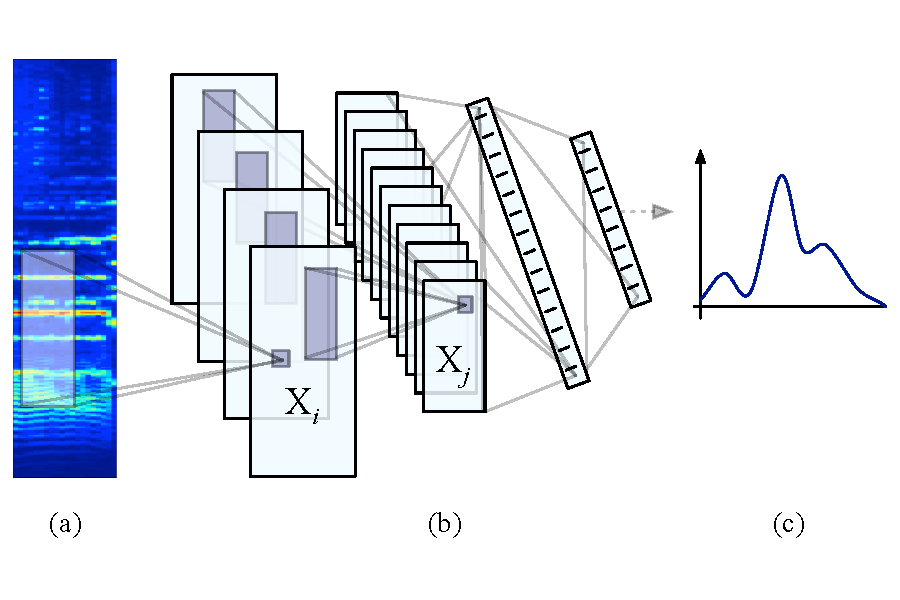
\includegraphics[width=3in]{pitch-CNN-prob}
\caption{The CNN Chord Recognition Architecture: A time-pitch tile (a) is input to a CNN (b), yielding a chord likelihood (c).}
\label{fig:system}
\end{figure}

this architecture is diagrammed in Figure \ref{fig:system}.


\subsubsection{Root-Invariant Classifier}
Take the data as-is, optimize the negative log-likelihood over the dataset.

$L(X^i, Y^i) = -ln(\mathcal{L}(X^i|Y^i))$

TODO: Observe that it learns a root invariant representation of qualities
Distance matrix between qualities
Ave vectors for same qualities in different roots


\subsubsection{Objective Function}
Take the data as-is, optimize the negative log-likelihood over the dataset.

$L(X^i, Y^i) = -ln(\mathcal{L}(X^i|Y^i))$

Then, at test time, apply likelihood scaling.
Consistent with ASR and other imbalanced learning problems.
Appropriately suited to HMM processing now


\subsubsection{Convolutional Dropout}
Here, we extend the principles of dropout, discussed in Chapter \ref{chp:deep_learning}, to 3D convolutions.
In the weight-matrix case, training with dropout effectively ignores activations of an transformed output, setting them to zero.
Considering each output coefficient as a measure of activation for a given ``feature'', the act of dropout can be interpretted as sub-sampling the feature extractors learned by the model.

By extension, there are two ways the same principle could be applied in the case of 3D convolutions.
One, the $i^{th}$ kernel, $W_i$, can be masked with probability $p$, resulting in the possibly empty feature map, $Z_i$:

\begin{equation}
Z_i = binomial(p) * h(X \circledast W_i + b_i) / (1.0 - p)
\end{equation}

\noindent where the output is also scaled by the complement of the probability.
Here, it is expected that each kernel learns a collection of feature extractors that, on average, work well together.
In the language of coadaptation, the tensor can be seen as a ``team'' of feature detectors, and as such correlations are broken up at this mid, as opposed to global, level.

Alternatively,


$L(X^i, Y^i) = -ln(\mathcal{L}(X^i|Y^i))$

Then, at test time, apply likelihood scaling.
Consistent with ASR and other imbalanced learning problems.
Appropriately suited to HMM processing now



\subsection{Evaluation and Metrics}
Classic metric is weighted chord symbol recall.
Give definitions, and point to MIREX.

However, this statistic is biased toward classes that occur most frequently.
Classically this has not proven to be an issue, because the vocabulary considered was restricted to the 24 Major/minor chords; and furthermore, when the data is rotated to be root-invariant, all statistics can be considered at the quality level.
When tackling an imbalanced learning problem, it can be just as important to consider the metrics that are used to quantify the system as the way that it is trained.

Binary classification, introduce various Type errors and confusion matrices.
Extending this to multiple classes, we can consider the class-wise precision and recall values over a square confusion matrix.
Need an image of a confusion matrix.
In this manner, precision is given by the columns, recall by the rows, and an f-score as a combination of the two.

Walkthrough example of why this is important.
Point out that we do not explicitly decide which measure is better, but acknowledge that systems that perform better on certain metrics may be more useful in different scenarios.


\subsection{Experimental Setup}

Resolve data to 24-maj/min + N
Test a variety of model complexities (number and size of kernels)





\section{Large Vocabulary Chord Estimation}



\subsection{Experimental Setup}



We get junk back! Heavy major bias, doesn't learn minority chords, as to be expected.

Demonstrate with toy example of parabola and Gaussian.

\subsection{Re-weighting the Data Distribution}

\subsubsection{Uniform Presentation}
The dataset is sampled such that the likelihood of drawing a datapoint with class $i$ from $K$ classes is $\frac{1}{K}$.

\subsubsection{Outlier Rejection}
Low intraclass likehood; a datapoint $X$ of class $i$ has a low likelihood of having label $Y$ for class $i$:
\begin{equation}
P(X^i | Y^i) \approx 0
\label{eq:outliers}
\end{equation}


\subsubsection{Avoiding Collisions}

High interclass confusion; a datapoint $X$ of class $i$ has a high likelihood of having label $Y$ for class $j$:

\begin{equation}
P(X^i | Y^j) \approx 1
\label{eq:collisions}
\end{equation}

\subsubsection{Curriculum Learning}
The dataset is chunked into sets and trained on progressively more difficult examples.

\subsection{Changing the Loss Function}

Observed problems with uniform presentation:
\begin{itemize}
\item Perhaps overly discriminative; cuts big gaps between near-neighbors, and makes it hard / impossible to post-filter the output.
\item Doesn't incorporate distribution bias; Majors are just more common than Maj6's.
\end{itemize}


\subsubsection{Limiting the Maximum Likelihood}

This seems to have pretty significant potential.
Prevents the optimization problem from running away, leaves hope for post-filtering.
Can ``accidentally'' get more things right by keeping the confusions closer together?

\begin{equation}
L(X^i, Y^i) = -ln(\mathcal{L}(X^i|Y^i)) + \lambda~max_j(\mathcal{L}(X^i|Y^j)), \text{for}~ j\in~K
\label{eq:collisions}
\end{equation}


\subsubsection{Margin Loss}
This keeps things closer.
Observed problem; error signal becomes much weaker as the training data is fit.
To circumvent this, it might be necessary to identify which data points should be revisited during training.
Margin of zero produces degenerate models. Information stops propagating.

\begin{equation}
L(X^i, Y^i) = \| max(m_{i,j} - (\mathcal{L}(X^i|Y^i) - \mathcal{L}(X^i|Y^j)), 0) \|_p, \text{where} j\neq~i
\label{eq:collisions}
\end{equation}


\subsubsection{Using the Distribution Prior}
The contribution of the loss from a given datapoint is weighted by its class frequency in the training set.
As-is, linear scale, logarithmic

\subsubsection{Substitution Matrix}
Build a language model determining the cost of confusing one chord with another; may be asymmetric.


\subsection{Alternative Representations}

\subsubsection{Predicting nodes on a decision tree}

\subsubsection{Generative Inference}




